\documentclass[tikz,border=8pt]{standalone}
\usepackage{lmodern}
\usetikzlibrary{arrows.meta,positioning,fit,backgrounds}
\definecolor{rmit}{HTML}{E04B2A}\tikzset{role/.style={draw,rounded corners,fill=rmit!12,minimum width=32mm,minimum height=13mm,align=center,font=\sffamily\small},op/.style={draw,rounded corners,fill=black!4,minimum width=34mm,minimum height=9mm,align=center,font=\sffamily\scriptsize},edge/.style={-{Latex[length=2mm]},thick}}
\begin{document}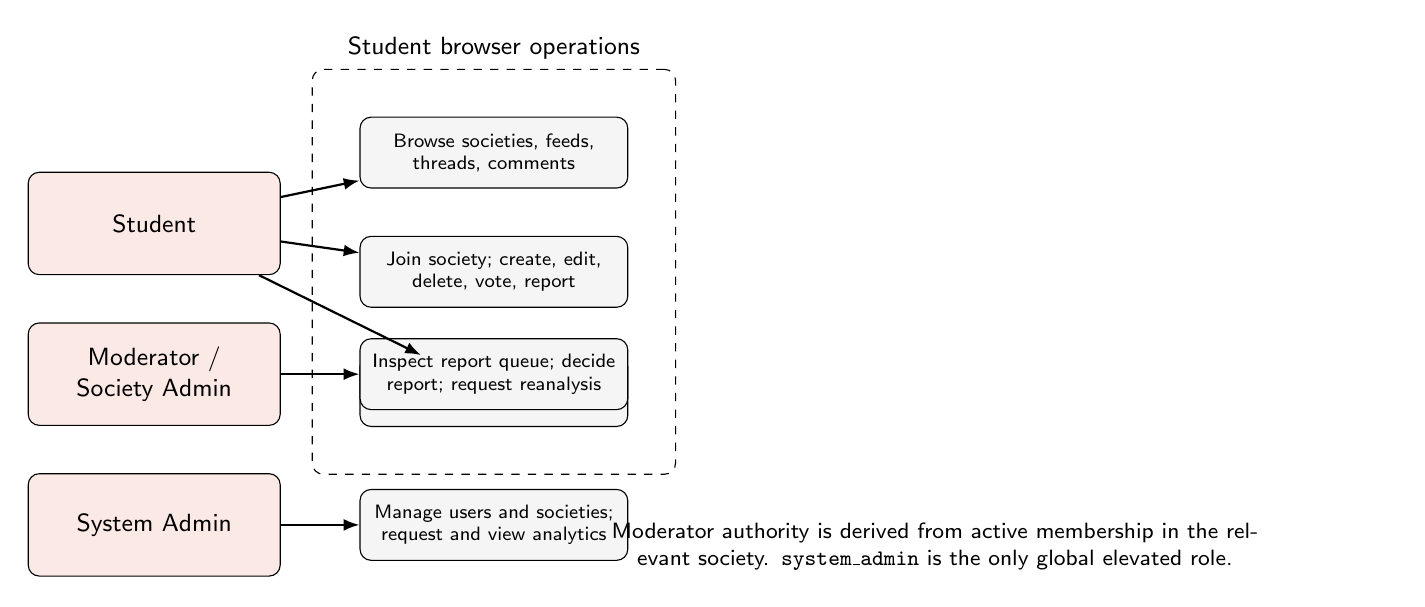
\begin{tikzpicture}[node distance=6mm and 10mm]
\node[role] (student) {Student};
\node[role,below=of student] (mod) {Moderator /\\Society Admin};
\node[role,below=of mod] (admin) {System Admin};
\node[op,right=of student,yshift=9mm] (browse) {Browse societies, feeds,\\threads, comments};
\node[op,below=of browse] (create) {Join society; create, edit,\\delete, vote, report};
\node[op,below=of create] (media) {Attach media; select\\verified location};
\node[op,right=of mod] (queue) {Inspect report queue; decide\\report; request reanalysis};
\node[op,right=of admin] (govern) {Manage users and societies;\\request and view analytics};
\draw[edge] (student) -- (browse);\draw[edge] (student) -- (create);\draw[edge] (student) -- (media);
\draw[edge] (mod) -- (queue);\draw[edge] (admin) -- (govern);
\node[draw,dashed,rounded corners,fit=(browse)(create)(media),inner sep=6mm,label={[font=\sffamily\small]above:Student browser operations}] {};
\node[font=\sffamily\footnotesize,align=center,below=11mm of media,xshift=56mm,text width=115mm] {Moderator authority is derived from active membership in the relevant society. \texttt{system\_admin} is the only global elevated role.};
\end{tikzpicture}\end{document}
